% !TEX root = ../main.tex





\begin{enumerate}

\import{./lib/}{1d_theorie_II_1} % Model EVB wagentje op een helling


\import{./lib/}{FV_T1_18p40} % Meerkeuze Oriëntatie versnelling

\import{./lib/}{1d_EVRB_II_1} % Formules EVRB
\import{./lib/}{1d_EVRB_I_1}
\import{./lib/}{1d_EVRB_I_2} % Bewijs formule gemiddelde snelheid
\import{./lib/}{1d_EVRB_I_3} % Eenvoudige algebra met formules EVB
\import{./lib/}{1d_EVRB_II_3} % Vliegtuig, Afstand gedurende 12e seconde

\import{./lib/}{1d_theorie_I_1}
\import{./lib/}{1d_theorie_I_2}
\import{./lib/}{1d_theorie_I_3}
\import{./lib/}{1d_theorie_II_2} % Ordenen snelheid en versnelling

\import{./lib/}{1d_denkvraag_II_1} % Verloop afstandsverschil vallende lichamen

\import{./lib/}{1d_EVB_grafiek_II_1}
\import{./lib/}{1d_EVB_grafiek_II_2}
\import{./lib/}{1d_EVB_grafiek_II_3}

\import{./lib/}{FV_T1_7p47}

\import{./lib/}{1d_EVRB_II_2} % Remmende trein

\import{./lib/}{1d_wis_II_1} % Formule v^2-v_0^2=2ax bewijzen
\import{./lib/}{1d_wis_II_2} % mk


\import{./lib/}{1d_valbeweging_I_1} %Verticale worp, standaard
\import{./lib/}{1d_valbeweging_I_2} % hoogte
\import{./lib/}{1d_valbeweging_I_3} % Misconceptie ...
\import{./lib/}{1d_valbeweging_II_1} % Parachutist
\import{./lib/}{1d_valbeweging_II_2} % FV 8 p. 86
\import{./lib/}{1d_valbeweging_II_3} %FV 3 p. 90
\import{./lib/}{1d_valbeweging_II_4} % Pelikaan die naar vis duikt
\import{./lib/}{1d_valbeweging_II_5} % Maximale hoogte op de maan
\import{./lib/}{1d_valbeweging_III_1} % Laatste 100 m
\import{./lib/}{1d_valbeweging_III_2} % FV 2 p. 92 Empire State Building
\import{./lib/}{1d_valbeweging_III_3} % Ziek man voor een raam
\import{./lib/}{1d_valbeweging_III_4} % Student gooit een sleutelbos
\import{./lib/}{1d_valbeweging_III_5} % formule voor maximale hoogte






\item Toon aan dat de positie en de snelheid van een eendimensionale beweging met constante versnelling, worden gegeven door de volgende functies:
\begin{eqnarray*}
x&=&x_0+v_0t+\frac{1}{2}at^2\\
v&=&v_0+at 
\end{eqnarray*}

\item Bewijs dat de plaatsfunctie $x(t)$ van een EVRB met versnelling $a$ gegeven wordt door:
\begin{eqnarray*}
x(t)=x_0+v_0(t-t_0)+\frac{1}{2}a(t-t_0)^2
\end{eqnarray*}

\item Toon aan dat voor een EVRB de snelheid als functie van de tijd wordt gegeven door:
\[v=v_0+a(t-t_0)\]



\item Laat zien dat voor een EVRB de volgende formule geldt:
\begin{eqnarray*}
x-x_0&=&\left(\frac{v+v_0}{2}\right)(t-t_0)
\end{eqnarray*}

\item Bewijs voor een EVRB de volgende formule voor de gemiddelde snelheid:
\begin{eqnarray*}
\overline{v}=\frac{v_0+v}{2}
\end{eqnarray*}


\item Bewijs dat de remweg van een met constante versnelling remmende auto, evenredig is met het kwadraat van de beginsnelheid.
\begin{oplossing}
\item[Bewijs]Bij het tot stilstand komen is de snelheid van de auto nul, zodat de tijd die hij hiervoor nodig heeft als volgt te vinden is:
\begin{eqnarray*}
v&=&0\\
&\Updownarrow&\\
v_0+at&=&0\\
&\Updownarrow&\\
t&=&-\frac{v_0}{a}
\end{eqnarray*}
Door deze tijd in de plaatsfunctie in te vullen, weten we welke afstand de auto heeft afgelegd gedurende het remmen.
\begin{eqnarray*}
x&=&v_0t+\frac{1}{2}at^2\\
&=&v_0\left(-\frac{v_0}{a}\right)+\frac{1}{2}a\left(-\frac{v_0}{a}\right)^2\\
&=&-\frac{v_0^2}{a}+\frac{v_0^2}{2a}\\
&=&-\frac{v_0^2}{2a}\\
\end{eqnarray*}
De factor $-\frac{1}{2a}$ is een (positieve, de versnelling is negatief) constante. De afgele afstand $x$ en het kwadraat van de beginsnelheid $v_0^2$ zijn dus recht evenredig. 
\end{oplossing}

\item Vanaf welke hoogte $x$ moet een lichaam vallen om met een snelheid $v$ de grond te bereiken?

\begin{oplossing}
	$x=\frac{v^2}{2g}$
\end{oplossing}



\item Een voorwerp beweegt op een rechte baan en
voert een eenparig versnelde beweging uit. Twee seconden na zijn
doorkomst in een referentiepunt R is de snelheid verdubbeld ten
opzichte van deze in R.
\newline
\newline
Dan was \'e\'en seconde na zijn doorkomst in het referentiepunt R de
snelheid:
\begin{enumerate}
\item 3/2 maal zo groot als deze in R.
\item 1/2 maal zo groot als deze in R.
\item 2/3 maal zo groot als deze in R.
\item $\sqrt{2}$ maal zo groot als deze in R.
\end{enumerate}
\footnote{antw. a}



\end{enumerate}




\cleardoublepage





\subsection{Vraagstukken}

\begin{enumerate}




\item Een automobilist rijdt gedurende $1,5\rm\,u$ tegen $80\rm\,km/h$ en daarna gedurende dezelfde tijdsduur tegen
$70\rm\,km/h$.
\begin{enumerate}
\item Wat is zijn gemiddelde snelheid?
\item Met welke snelheid had hij moeten rijden om met een constante snelheid hetzelfde traject in dezelfde tijd af te leggen?
\end{enumerate}

\item Een automobilist legt $120\rm\,km$ af. De eerste helft van de weg legt hij af tegen $90\rm\,km/h$, de tweede helft tegen $120\rm\,km/h$. Wat is zijn gemiddelde snelheid?

\item Een fietser legt een bepaalde afstand af over een zekere tijd. Gedurende de eerste helft van de tijd houdt hij constant een snelheid $v_1$ aan, gedurende de tweede helft een snelheid $v_2$. Wat is zijn gemiddelde snelheid over het totale tijdsinterval?
\begin{oplossing}
\footnote{$\overline{v}=\frac{v_1+v_2}{2}$}
\end{oplossing}

\item Een fietser legt een bepaalde afstand af over een zekere tijd. Gedurende de eerste helft van de af te leggen afstand houdt hij constant een snelheid $v_1$ aan, gedurende de tweede helft een snelheid $v_2$. Wat is zijn gemiddelde snelheid over het totale tijdsinterval? 
\begin{oplossing}
\footnote{$\overline{v}=\frac{2v_1v_2}{v_1+v_2}$}
\end{oplossing}


\item Als je met de fiets heen en terug naar school rijdt en in het heengaan tegenwind en in het terugkeren rugwind hebt, compenseert dat dan mekaar precies?

Stel om dit op te lossen dat de weg rechtlijnig is. Bereken je gemiddelde snelheid over het traject heen en terug en vergelijk die met de snelheid die je zonder wind zou halen. Neem aan dat je normaal $10~\rm km/h$ zou fietsen, maar door de wind win of verlies je $2~\rm km/h$.
\begin{enumerate}
\item Nee, je hebt netto een nadeel vanwege de tegenwind.
\item Nee, je hebt netto een voordeel vanwege de rugwind.
\item Ja, de afstand heen is de afstand terug, dus het is net alsof je helemaal geen wind had.
\end{enumerate}
\begin{oplossing}
Antwoord (a) is juist.
\end{oplossing}

\item Een bowlingbal die met een constante snelheid voort rolt, raakt de kegels aan het einde van een kegelbaan van $16,5\rm\,m$ lengte. De werper hoorde het geluid waarmee de bal op de kegels botst $2,5\rm\,s$ nadat hij de bal losliet. Welke snelheid had de bal? De snelheid van het geluid is $343\rm\,m/s$. 
\begin{oplossing}
$v_1=\frac{x_1}{t_2-\frac{x_1}{v_2}}=6,73\rm\,m/s$
\end{oplossing}

\item Twee personen A en B voeren op dezelfde rechte en vanuit dezelfde beginstand een eenparige beweging uit. A vertrekt $100\rm\,s$ eerder dan B. Met een snelheid die dubbel zo groot is als die van A haalt B, op $400\rm\,m$ van het vertrekpunt, A in. Bereken beide snelheden en stel ze grafisch voor.
%\begin{oplossing}
%\item[gegeven]$x_0=1,00\cdot10^3\rm\,m$\newline$t_0=100\rm\,s$\newline$v_b=-2v_a$\newline$x=400\rm\,m$
%\item[gevraagd]$v_a$, $v_b$
%\item[oplossing]De bewegingsvergelijkingen voor A en B worden gegeven door:
%\begin{eqnarray}
%A:\qquad x&=&v_at \label{verg A}\\
%B:\qquad x&=&x_0+v_b(t-t_0)\nonumber\\
%&=&x_0-2v_a(t-t_0) \label{verg B}
%\end{eqnarray}
%De grafiek van beide functies ziet er als volgt uit:
%\begin{figure}[h]
%\centering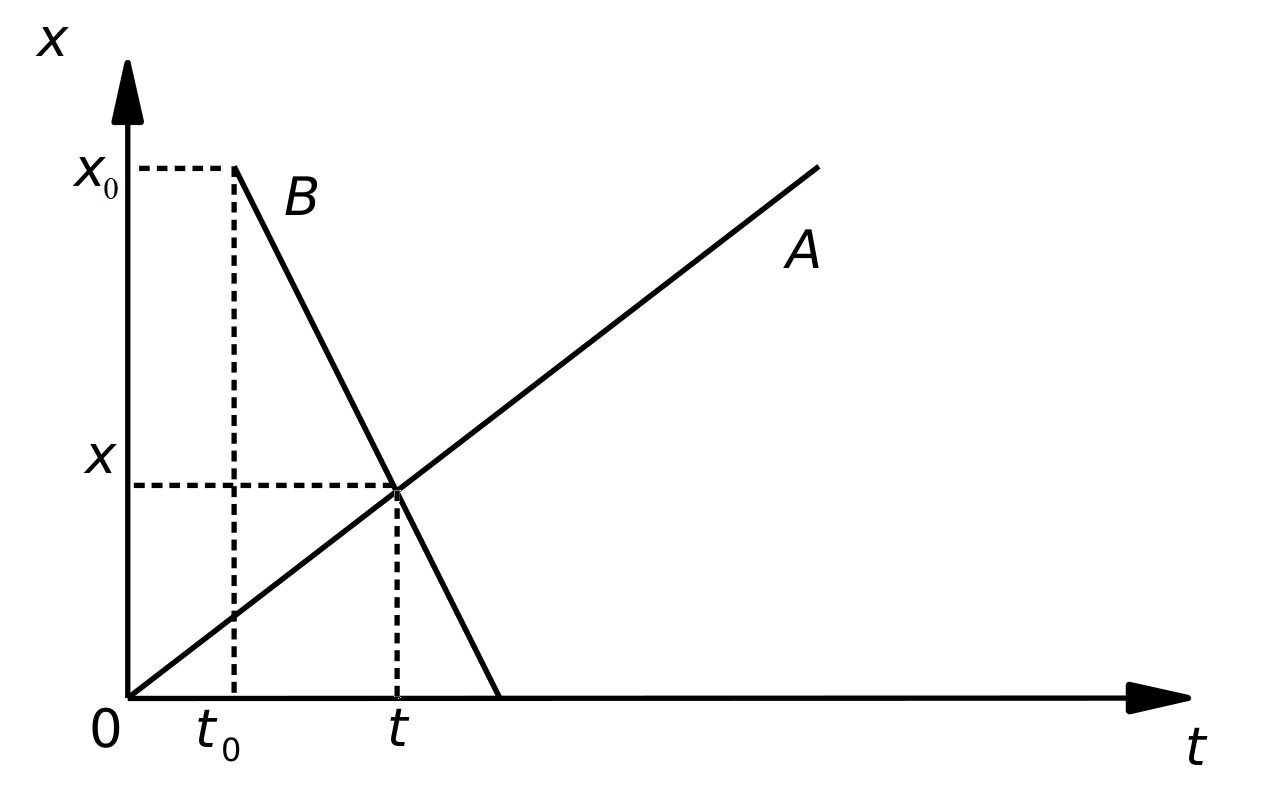
\includegraphics[width=0.6\textwidth]{38p40}
%\end{figure}
%\newline
%Als we voor $x$ de ontmoetingsplaats van $400\rm\,m$ nemen, hebben we twee vergelijkingen (\ref{verg A}), (\ref{verg B}) en twee onbekenden $t$, $v_a$. Dit kunnen we oplossen door een variabele te substitueren. We nemen de tijd, $(\ref{verg A})\Leftrightarrow t=\frac{x}{v_a}$ en substitueren deze in vergelijking (\ref{verg B}):
%\begin{eqnarray*}
%x&=&x_0-2v_a(t-t_0)\\
%&=&x_0-2v_a\left(\frac{x}{v_a}-t_0\right)\\
%&\Updownarrow&\\
%v_a&=&\frac{3x-x_0}{2t_0}=1,0\rm\,m/s
%\end{eqnarray*}
%En de snelheid van B:
%\begin{equation}
% v_b=-2v_a=\frac{x_0-3x}{t_0}=-2,0\rm\,m/s
%\end{equation} 
%\end{oplossing}


\item Een vliegtuig moet minstens een snelheid van $108\rm\,km/h$ hebben om te kunnen opstijgen. Indien de schroeven aan het toestel een versnelling van $1,50\rm\,m/s^2$ geven, hoe lang moet de startbaan dan minstens zijn? 
%\begin{oplossing}
%\footnote{$x=\frac{v^2}{2a}=300\rm\,m$}
%\end{oplossing}
\begin{oplossing}
\item[gegeven]$v=30,0\rm\,m/s$\newline$a=1,50\rm\,m/s^2$
\item[gevraagd]$x$
\item[oplossing]Doordat we de versnelling van het vliegtuig kennen en de snelheid die het moet bereiken, kunnen we de tijd die het vliegtuig hiervoor nodig heeft, gemakkelijke berekenen met de formule $v=v_0+at$ voor de snelheid van een EVRB:
\begin{eqnarray*}
t=\frac{v}{a}
\end{eqnarray*}
De afstand die in deze tijd wordt afgelegd, kunnen we berekenen doordat we de gemiddelde snelheid kennen\footnote{De benodigde afstand kunnen we evenzeer berekenen met de formule $x=x_0+v_0+\frac{1}{2}at^2$ door de tijd in te vullen.}:
\begin{eqnarray*}
x&=&\frac{v_0+v}{2}\cdot t\\
&=&\frac{v}{2}\cdot\frac{v}{a}\\
&=&\frac{v^2}{2a}
\end{eqnarray*}
De startbaan moet dus minstens $300\rm\,m$ lang zijn.
\end{oplossing}

\item Op een bevroren meer komt een glijdende hockeyschijf na $200\rm\,m$ tot stilstand. Als zijn initi\"ele snelheid $3,00\rm\,m/s$ was, bepaal dan
\begin{enumerate}
\item de versnelling in de veronderstelling dat deze constant is,
\item de tijd die de schijf nodig heeft om tot stilstand te komen.
\end{enumerate}
\begin{oplossing}
	$a=\frac{v_0^2}{2x}=0,0225\rm\,m/s^2$; $t=\frac{2x}{v_0}=133,33\rm\,s$
\end{oplossing}

\item Een bootje vaart met een snelheid van $36,0\rm\,km/h$ een eerste tijdopnemer voorbij en drijft daarna eenparig zijn snelheid op. Na $20,0\rm\,s$ komt het voorbij een tweede tijdopnemer met een snelheid van $90,0\rm\,km/h$. Bereken de versnelling van het bootje en de afstand tussen beide tijdopnemers.
\begin{oplossing}
\newline
$a=\frac{v-v_0}{t-t_0}=0,750\rm\,m/s^2$, $x-x_0=\left(\frac{v_0+v}{2}\right)(t-t_0)=350\rm\,m$
\end{oplossing}

\item Een auto begint te remmen als hij zich $35\rm\,m$ van een hindernis bevindt. Zijn snelheid op dat moment is $54\rm\,km/h$. Na $4,0\rm\,s$ botst hij tegen de hindernis. Bereken de snelheid waarmee hij de hindernis raakt en zijn constante versnelling gedurende de remweg.
\begin{oplossing}
$a=\frac{2(x-v_0t)}{t^2}=-3,125\rm\,m/s^2$, $v=\frac{2x}{t}-v_0=2,5\rm\,m/s$
\end{oplossing}
\begin{oplossing}
\item[gegeven]$x=35\rm\,m$\newline$v_0=15\rm\,m/s$\newline$t=4,0\rm\,s$
\item[gevraagd]$a, v$
\item[oplossing]Uit de plaatsfunctie kunnen we de versnelling halen:
\begin{eqnarray*}
x&=&v_0t+\frac{1}{2}at^2\\
&\Updownarrow&\\
a&=&\frac{2x-2v_0t}{t^2}
\end{eqnarray*}
Substitutie van de versnelling in de snelheidsfunctie levert:\footnote{Een andere (snellere) mogelijkheid is de snelheid uit $x=\frac{v_0+v}{2}t$ halen.}
\begin{eqnarray*}
v&=&v_0+at\\
&=&v_0+\left(\frac{2x-2v_0t}{t^2}\right)t\\
&=&\frac{2x}{t}-v_0\\
&=&2,5\rm\,m/s
\end{eqnarray*}
\end{oplossing}

\item Twee fietsers vertrekken gelijktijdig om
een afstand van $200\rm\,m$ af te leggen. De eerste rijdt met een
constante snelheid van $4,0\rm\,m/s$, terwijl de tweede vertrekt met
een snelheid van $1,00\rm\,m/s$ en de afstand van $200\rm\,m$ met
een EVRB met een versnelling van $0,20\rm\,m/s^2$ aflegt. Waar zal
de tweede fietser de eerste inhalen en wanneer?
\begin{oplossing}
\newline
$t=\frac{2(v_a-v_{b,0})}{a}=30\rm\,s$,
$x=v_at=\frac{2v_a(v_a-v_{b,0})}{a}=120\rm\,m$
\end{oplossing}

\item Laat zien dat voor een EVRB de volgende formules gelden:
\begin{eqnarray*}
x-x_0=\left(\frac{v+v_0}{2}\right)(t-t_0)\\
v^2=v_0^2+2a(x-x_0)\\
x-x_0=v(t-t_0)-\frac{1}{2}a(t-t_0)^2
\end{eqnarray*}

\item Een trein verlaat het station a en rijdt
naar het station b, op $15,0~\rm km$ van a gelegen. De eerste
$1000~\rm m$ worden afgelegd met een EVRB en de verkregen snelheid
is $72,0~\rm km/h$. Die snelheid blijft constant tot op $250~\rm m$
van b. Hier begint de trein te vertragen. Wanneer komt hij in
station b toe? Maak de $v(t)$-grafiek.










\item 
\begin{minipage}[t]{0.5\textwidth}
Een deeltje beschrijft een eendimensionale beweging op de $x$-as. De positie als functie van de tijd is hiernaast weergegeven in een $x(t)$-diagram. Duid de onderstaande grafiek aan die het best het verloop weergeeft van de snelheidscomponent $v$ van dat deeltje als functie van de tijd. 
\end{minipage}
\hspace{0.1\textwidth}
\begin{minipage}[t]{0.3\textwidth}
\raisebox{-5cm}{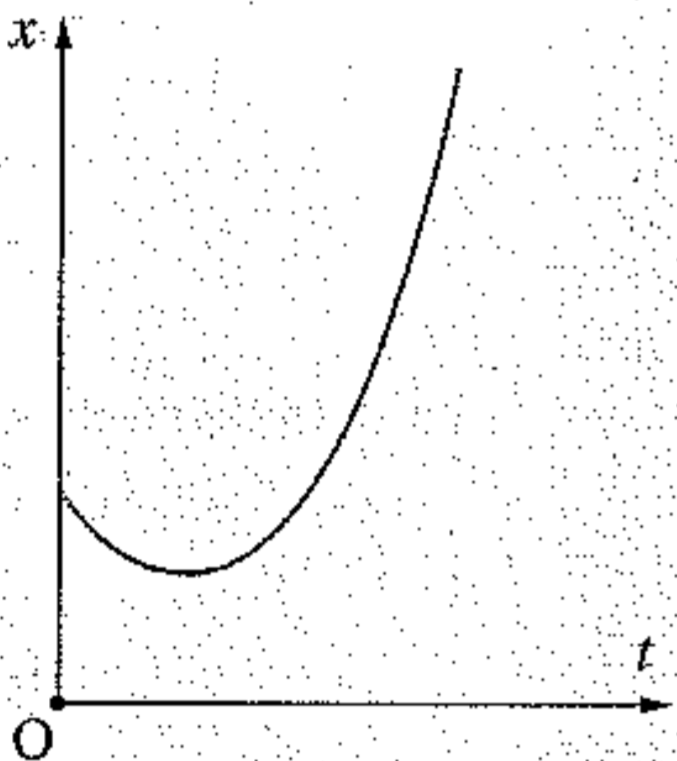
\includegraphics[width=\textwidth]{snelheidsverloop_o}}
\end{minipage}
\begin{figure}[h]
\begin{flushright}
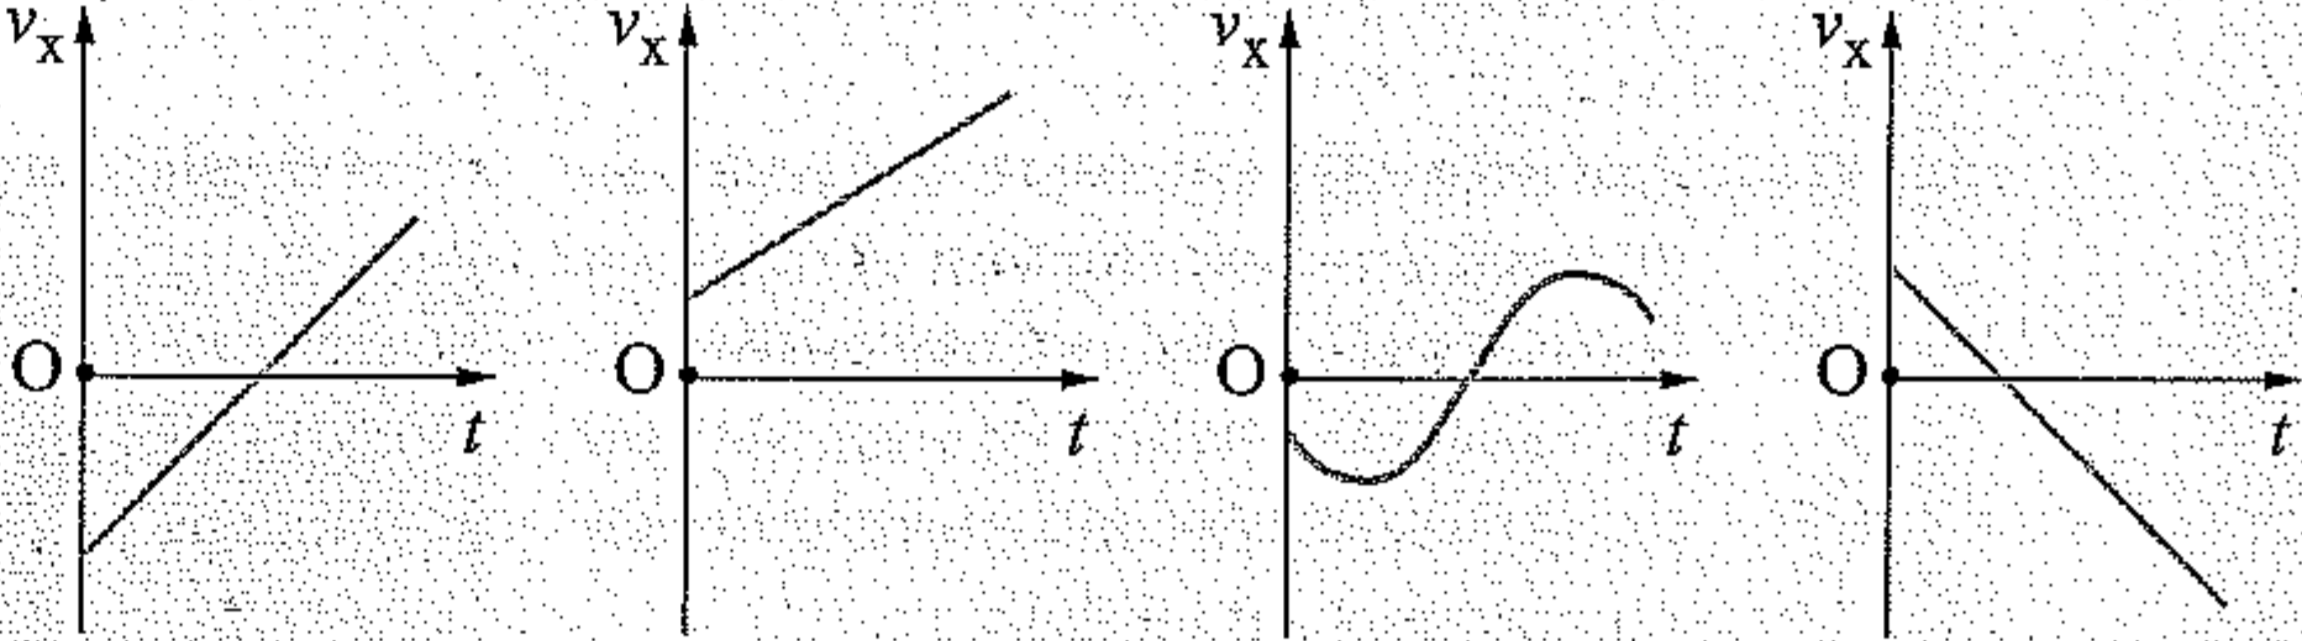
\includegraphics[width=0.93\textwidth]{snelheidsverloop}
\end{flushright}
\end{figure}

\item 
\begin{minipage}[t]{0.6\textwidth}
Een deeltje beweegt in de zin van de $x$-as. De nevenstaande grafiek geeft aan hoe de grootte van de snelheid verandert als functie van de tijd.
\begin{enumerate}
\item De afstand afgelegd na $15\rm\,s$ bedraagt:
\newline
\begin{tabularx}{\textwidth}{XXXX}
$30\rm\,m$&$120\rm\,m$&$150\rm\,m$&$240\rm\,m$
\end{tabularx}
\item Na $30\rm\,s$ heeft het deeltje een welbepaalde afstand afgelegd. Hoe groot zou de constante snelheid van het deeltje moeten zijn om in $30\rm\,s$ dezelfde afstand af te leggen?
\newline
\begin{tabularx}{\textwidth}{XXXX}
$0,0\rm\,m/s$&$§6,0\rm\,m/s$&$8,0\rm\,m/s$&$12\rm\,m/s$
\end{tabularx}
\end{enumerate}
\end{minipage}
\hspace{2mm}
\begin{minipage}[t]{0.3\textwidth}
\raisebox{-5cm}{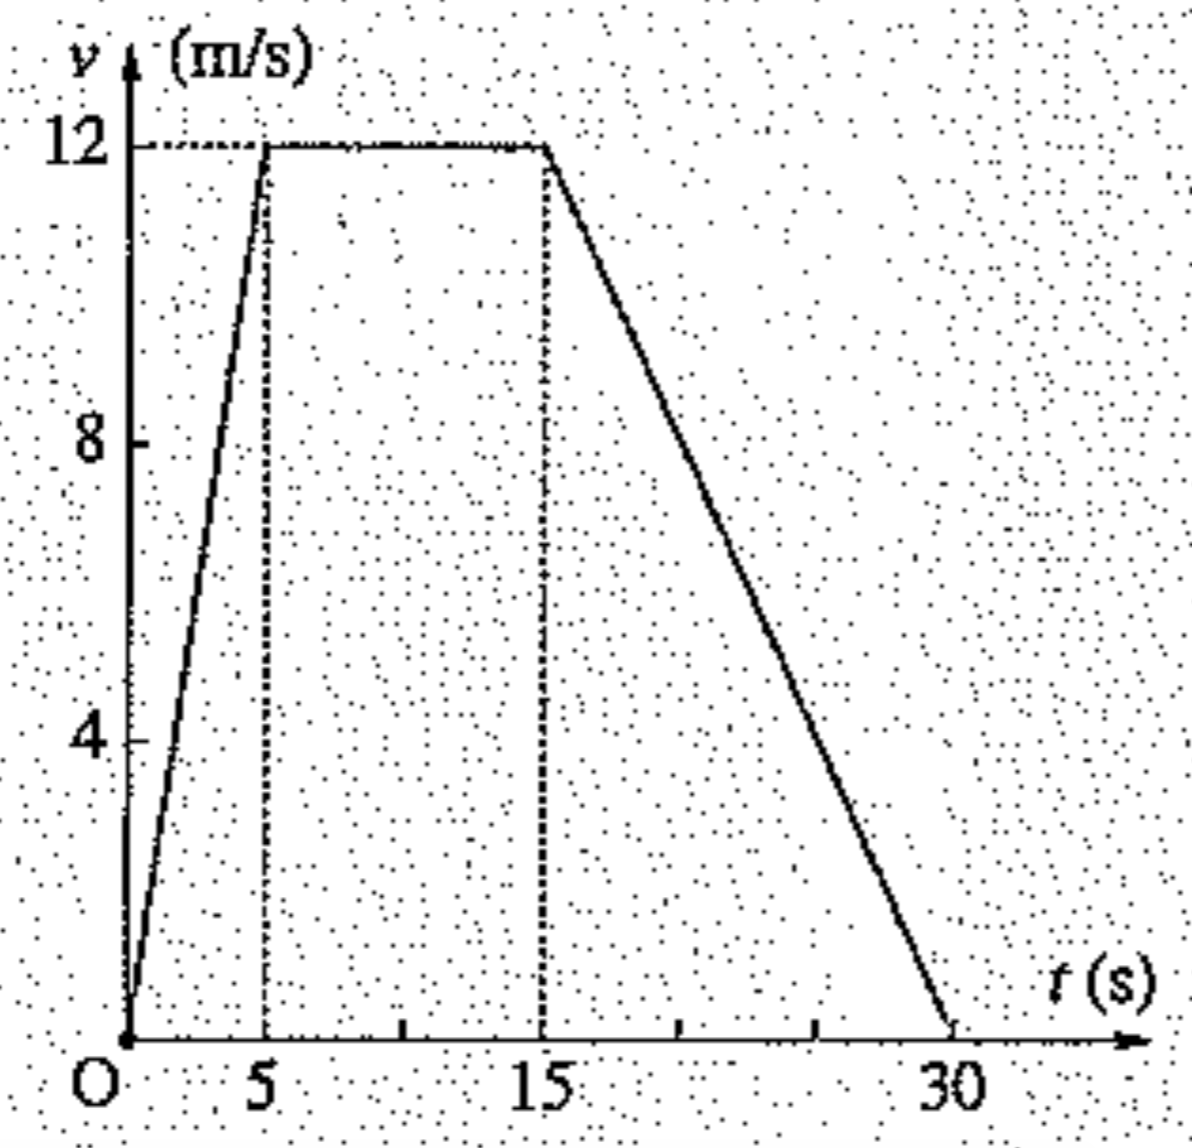
\includegraphics[width=\textwidth]{snelheidsverloop_2_o}}
\end{minipage}
\begin{enumerate}
\setcounter{enumii}{2}
\item Het verloop van de versnellingscomponent van het deeltje wordt kwalitatief voorgesteld op figuur:
\begin{figure}[h]
\begin{flushright}
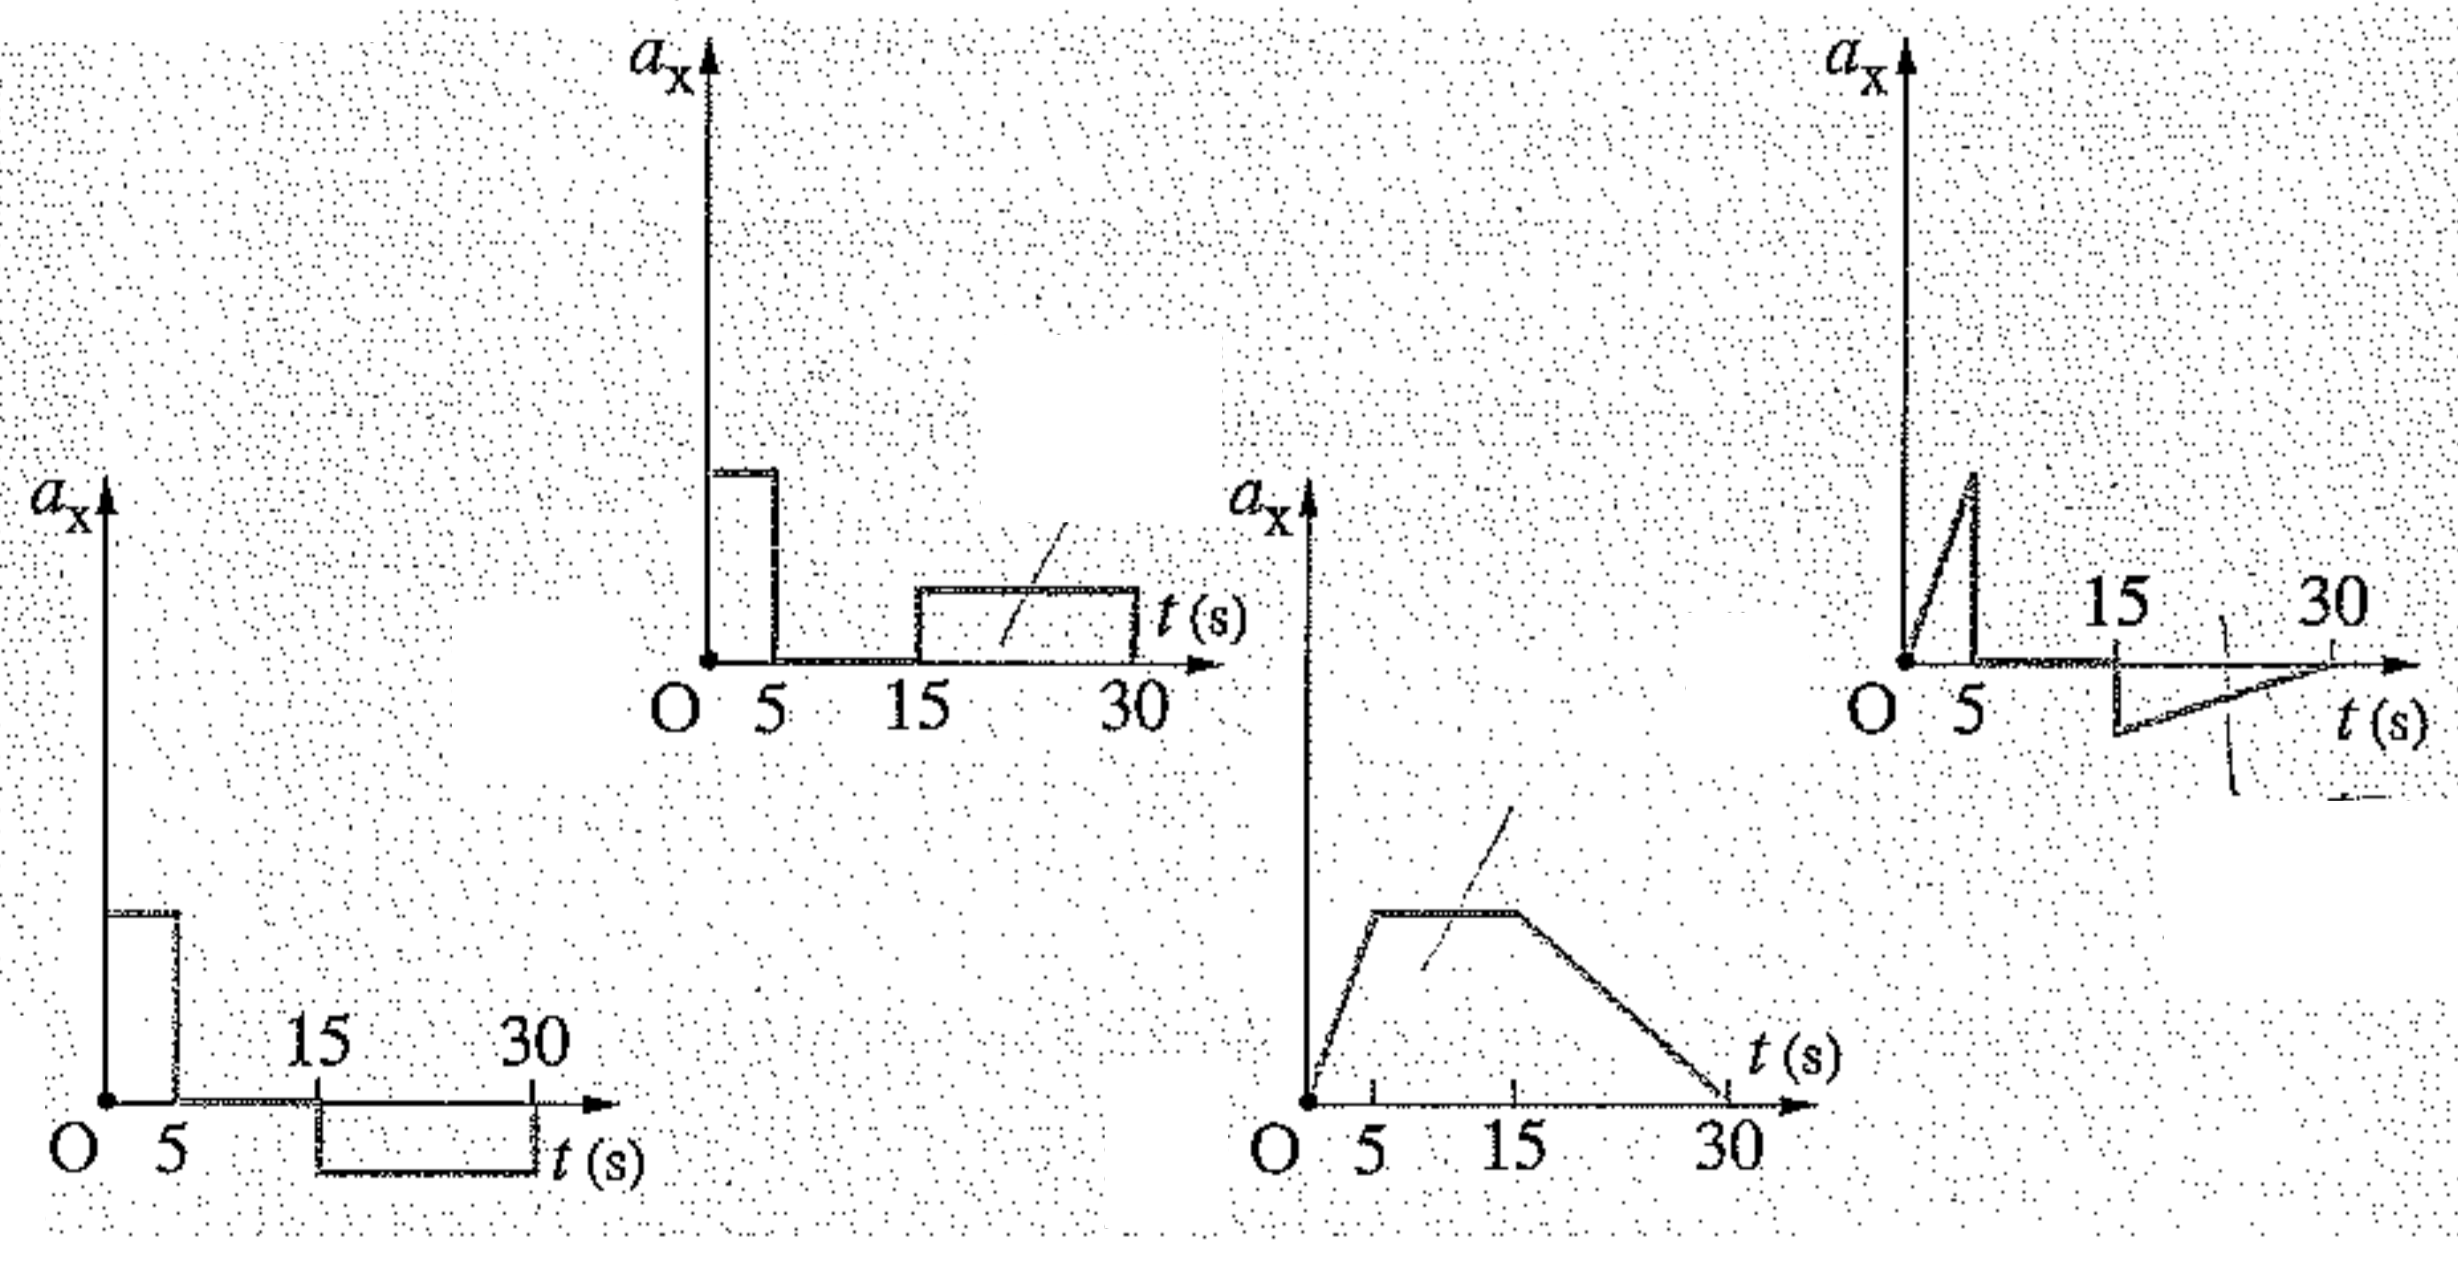
\includegraphics[width=0.93\textwidth]{snelheidsverloop_2}
\end{flushright}
\end{figure}
\end{enumerate}

\item Toon aan dat voor het stoptraject ($x_s$) van een auto de volgende vergelijking geldt:
\begin{eqnarray*}
x_s&=&v_0t_r-\frac{v_0^2}{2a}
\end{eqnarray*}
waarin $v_0$ de beginsnelheid van de auto is, $t_r$ de reactietijd van de bestuurder, en $a$ de vertraging (negatief).
\newline
\newline
Maak een $x(t)-,\,v(t)-$ en een $a(t)-$grafiek van de beweging.
\begin{oplossing}
\newline
\newline
Het stoptraject bestaat uit twee delen: gedurende de reactietijd blijft de bestuurder met de gegeven snelheid verder rijden om vervolgens, van zodra hij de rem indrukt, effectief te beginnen remmen. Het stoptraject bestaat uit de som van de afstanden afgelegd gedurende die twee delen:
\begin{eqnarray*}
x_s=\Delta x_{\mathrm{reactie}}+\Delta x_{\mathrm{rem}}
\end{eqnarray*}
Omdat de snelheid gedurende de reactietijd constant is, wordt de afstand die hier wordt afgelegd gegeven door $\Delta x_{\mathrm{reactie}}=v_0t_r$. In het tweede deel bestaat de beweging uit een rechtlijnige beweging met een constante versnelling. Omdat de tijd om van een gegeven snelheid tot stilstand te komen, wordt gegeven door $\Delta t=-\frac{v_0}{a}$ en de gemiddelde snelheid door $\frac{v_0}{2}$, wordt de afstand gegeven door $\Delta x_{\mathrm{rem}}=\bar{v}\Delta t=-\frac{v_0}{a}\frac{v_0}{2}=-\frac{v_0^2}{2a}$. We vinden het stoptraject als de som van de twee afstanden.
%$\Delta x_{rem}=v_0\Delta t+\frac{1}{2}a\Delta t^2$.
\end{oplossing}



\item (III) Maggie en Jennifer lopen de \SI{100}{m}. Beiden doen ze er exact 10,2 se\-conden over. Met een eenparige versnelling bereikt Maggie na \SI{2}{s} haar maximale snelheid, Jennifer doet dat na \SI{3}{s}. Hun maximale snelheden houden ze aan voor de rest van de wedstrijd.
\begin{enumerate}
\item Wat zijn hun maximale snelheden?
\item Wat is de versnelling van iedere sprinter?
\item Wie heeft er voorsprong na \SI{6}{s}, en hoeveel?
\end{enumerate}
\begin{oplossing}
\footnote{antw. $v_1=\frac{2x_2}{2t_2-t_1}$;
$a=\frac{2x_2}{(2t_2-t_1)t_1}$;
$x_M-x_J=\frac{2x_2}{2t_2-t_{1,M}}(t-\frac{t_{1,M}}{2})-\frac{2x_2}{2t_2-t_{1,J}}(t-\frac{t_{1,J}}{2})$}
\end{oplossing}

\item Welke afstand wordt er door een bungeespringer na een vrije val van $2,5\rm\,s$ afgelegd?
\begin{oplossing}
\footnote{$x=\frac{1}{2}gt^2=31\rm\,m$}
\end{oplossing}







\item Men laat een steen vallen van een $44,1\rm\,m$ hoge brug. $1\rm\,s$ later werpt men een tweede steen verticaal naar beneden. Beide raken gelijk het wateroppervlak. Zoek de beginsnelheid van de tweede steen.
\begin{oplossing}
\footnote{antw. $12,26\rm\,m/s$}
\end{oplossing}












\item (III) Germien laat een steen in een diepe put vallen. Na 2,6 seconden hoort ze dat de steen de bodem heeft geraakt. Hoe diep is de put? Neem voor de snelheid van het geluid $343\rm\,m/s$.




\begin{oplossing}
\begin{enumerate}
\item[\textit{gegeven}]$v_0=50\rm\,m/s$\newline$a=-30\rm\,m/s^2$\newline$v=5,0\rm\,m/s$
\item[\textit{gevraagd}]$x$
\item[\textit{oplossing}]Aangezien we de versnelling en begin- en eindsnelheid kennen, kunnen we de tijd die nodig is om de eindsnelheid te bereiken, berekenen:
\begin{eqnarray*}
v=v_0+at&\Leftrightarrow&t=\frac{v-v_0}{a}
\end{eqnarray*}
De afgelegde afstand is dan met gemiddelde snelheid te bepalen:
\begin{eqnarray*}
x&=&\overline{v}t\\
&=&\frac{v_0+v}{2}\cdot\frac{v-v_0}{a}\\
&=&\frac{v^2-v_0^2}{2a}\\
&=&41,25\rm\,m
\end{eqnarray*}
\end{enumerate}
\end{oplossing}
	



\item Een auto die $90\rm\,km/h$ rijdt, ligt $100\rm\,m$ achter op een vrachtwagen die $75\rm\,km/h$ rijdt. Hoeveel tijd kost het de auto om de vrachtwagen in te halen? 
\begin{oplossing}
\footnote{$t=\frac{x_0}{v_a-v_v}=24\rm\,s$}
\end{oplossing}

\item De snelheid van een trein verandert eenparig in 2 minuten van $20\rm\,km/h$ tot $30\rm\,km/h$. De trein rijdt gedurende die tijd over een rechte spoorlijn.
\begin{enumerate}
    \item Bepaal de versnelling.
    \item Bepaal de afstand die de trein heeft afgelegd gedurende deze 2 minuten.
\end{enumerate}

\item Een auto trekt in $5,0\rm\,s$ op van $10\rm\,m/s$ naar $25\rm\,m/s$. Wat was de versnelling in de veronderstelling dat de auto een EVRB ondergaat? Welke afstand legde de auto in deze periode af?
\begin{oplossing}
\newline
$a=\frac{v-v_0}{t-t_0}=3\rm\,m/s$,
$x-x_0=\left(\frac{v_0+v}{2}\right)(t-t_0)=87,5\rm\,m$
\end{oplossing}

\item Bij het katapulteren van vliegtuigen wordt een startbaan van
$25,0\rm\,m$ gebruikt, die door het vliegtuig eenparig versneld in
$1,00\rm\,s$ wordt doorlopen. Zoek zijn versnelling en de snelheid
waarmee het de baan verlaat.

\item Een auto trekt op tot $100\rm\,km/h$ in $6,0\rm\,s$. Als hij
dat doet op een rechte baan met constante versnelling, welke afstand
is er dan hiervoor nodig?~\footnote{antw.
$a=\frac{v}{t}=4,63\rm\,m/s^2$, $x=\frac{vt}{2}=83,3\rm\,m$}

\item Een auto vertrekt vanuit rust en bereikt na $3,0\rm\,km$ een snelheid van $450\rm\,km/h$ We onderstellen de versnelling constant en de baan recht. Bereken de versnelling en de tijd, nodig om die $3,0\rm\,km$ af te leggen.
\begin{oplossing}
\footnote{$t=\frac{2x}{v}=48\rm\,s$, $a=\frac{v^2}{2x}=2,6\rm\,m/s^2$}
\item[gegeven]$x=3000\rm\,m$\newline $v=125\rm\,m/s$
\item[gevraagd]$a$, $t$
\item[oplossing]Omdat voor een EVRB de gemiddelde snelheid gegeven wordt door $\overline{v}=\frac{v_0+v}{2}$ en we de afgelegde afstand kennen, kunnen we de benodigde tijd gemakkelijk vinden. We kiezen $t_0=0$, $x_0=0$. De beginsnelheid is nul zodat:
\begin{eqnarray*}
\Delta x &=& \overline{v}\Delta t \\
&\Downarrow & \\
t &=& \frac{x}{\left(\frac{v}{2}\right)} = \frac{2x}{v}
\end{eqnarray*}
Invullen van de gegevens levert een tijd van $48\rm\,s$. Met het formuletje voor de snelheid vinden we de versnelling door de tijd te substitueren:
\begin{eqnarray*}
v &=& at \\
&\Updownarrow&\\
a &=& \frac{v}{t}=\frac{v}{\left(\frac{2x}{v}\right)}\\
&=& \frac{v^2}{2x}
\end{eqnarray*}
Invullen van de gegeven grootheden levert een versnelling van $2,6\rm\,m/s^2$.
\end{oplossing}

\item Een vliegtuig landt met een snelheid van $100\rm\,m/s$. Op de ladingsbaan heeft het een vertraging van $5,0\rm\,m/s^2$. Welke afstand heeft het vliegtuig nodig om tot stilstand te komen?

\item Een trein vertrekt uit een station en rijdt met een eenparig
versnelde beweging waarvan de versnelling $0,50\rm\,m/s^2$ bedraagt.
Hoe groot is de afstand die de trein heeft afgelegd als zijn
snelheid $72,0\rm\,km/h$ bedraagt?



\item Een puntmassa voert een eenparig veranderlijke rechtlijnige
beweging uit over het tijdsinterval [$0\rm\,s$,$2\rm\,s$] met
beginsnelheid en beginpositie van respectievelijk $0\rm\,m/s$ en
$0\rm\,m$. De versnelling is $3\rm\,m/s^2$. Waarom kan je
onmiddellijk stellen dat als in het tijdsinterval de tijd half om
is, de puntmassa nog niet halfweg is?
\begin{enumerate}
    \item Breng, zoals de opgelegde werkwijze bij het oplossen van
    vraag\-stuk\-ken vereist, zowel het gegeven als het gevraagde (hier
    het te bewijzen) in symbolen.
    \item Leg in woorden uit op welke manier je onmiddellijk kan
    inzien dat het te bewijzen juist is.
    \item Controleer het te bewijzen via de numerieke waarden van
    dit vraagstuk.
    \item Geef nu het bewijs.
\end{enumerate}

\item Een puntmassa beweegt volgens een eenparig veranderlijke
rechtlijnige beweging. De puntmassa heeft een beginsnelheid $v_0$ en
een snelheid $v$ op het tijdstip $t$. Wat is zijn gemiddelde
snelheid over het interval [0,$t$]?

\item Een sprinter legt de 100 meter af in
$12,0~\rm s$. Het snelheidsverloop van de sprinter is in
onderstaande figuur grafisch voorgesteld.
\begin{figure}[h]
\begin{center}
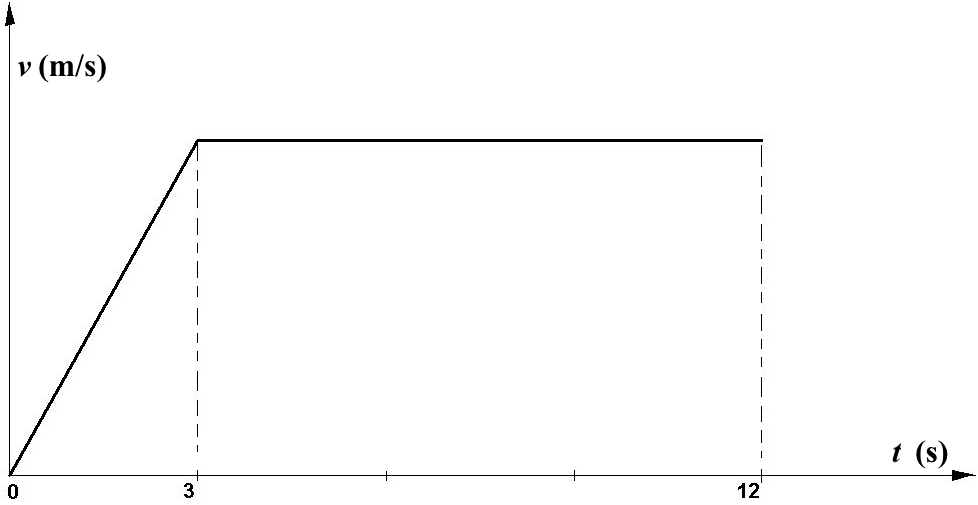
\includegraphics[width=0.5\textwidth, angle=0]{sprinter}
\end{center}
\end{figure}
\newline
Bereken
\begin{enumerate}
\item de constante snelheid die de sprinter gedurende de laatste 9
seconden aanhoudt,
\item de afstand die de sprinter gedurende de eerste 3 seconden
aflegt,
\item de versnelling die de sprinter heeft gedurende de eerste 3 seconden.
\end{enumerate}

\item Een ruimtevoertuig met een constante versnelling verhoogt
zijn snelheid van $65\rm\,m/s$ op $t=0\rm\,s$, tot $162\rm\,m/s$ op
$t=10,0\rm\,s$. Welke afstand legde dit voertuig af tussen
$t=2,0\rm\,s$ en $t=6,0\rm\,s$?~\footnote{antw.
$x_2-x_1=v_0(t_2-t_1)+\frac{1}{2}\left(\frac{v-v_0}{t}\right)(t_2^2-t_1^2)=415\rm\,m$}



%\item Toon aan dat voor het stoptraject ($x_s$) van een auto de volgende vergelijking geldt:
%\begin{eqnarray*}
%x_s&=&v_0t_r-\frac{v_0^2}{2a}
%\end{eqnarray*}
%waarin $v_0$ de beginsnelheid van de auto is, $t_r$ de reactietijd van de bestuurder, en $a$ de vertraging (negatief).
%\newline
%\newline
%Maak een $x(t)-,\,v(t)-$ en een $a(t)-$grafiek van de beweging.

\item Een onopgemerkte politieauto met
een constante snelheid van 90 km/h wordt ingehaald door een
snelheidsovertreder die 144 km/h rijdt. Precies 1,00 s nadat de
snelheidsovertreder passeert, geeft de politieagent plankgas; stel
dat de politieauto een versnelling heeft van $2,00\rm\,m/s^2$.
\begin{enumerate}
\item Hoe lang duurt het voordat de agent de snelheidsovertreder
(die met een constante snelheid blijft rijden) heeft ingehaald?
\item Wat is zijn snelheid op dat moment?
\item Schets nauwkeurig en net de $x(t)-,v(t)-$ en $a(t)-$grafieken.
Behandel de politieauto en de overtreder steeds in dezelfde grafiek.
\item Vind een (algebra\"ische) formule voor de gemiddelde snelheid $\overline{v}_{12}$ in
functie van de gegeven grootheden, tussen het tijdstip waarop de
agent begint te versnellen en het tijdstip waarop hij de overtreder
inhaalt.
\end{enumerate}

\item Een onopgemerkte politieauto met een constante snelheid van $95\rm\,km/h$ wordt ingehaald door een snelheidsovertreder die $140\rm\,km/h$ rijdt. Precies $1,00\rm\,s$ nadat de snelheidsovertreder passeert, geeft de politieagent plankgas; stel dat de politieauto een versnelling heeft van $2,00\rm\,m/s^2$, hoe lang duurt het dan voordat de agent de snelheidsovertreder (die met een constante snelheid blijft rijden) heeft ingehaald? 


\item Twee fietsers vertrekken gelijktijdig om een afstand van $500\rm\,m$ af te leggen. De eerste rijdt met een constante snelheid van $5,0\rm\,m/s$, terwijl de tweede het traject aflegt met een EVRB waarvan de beginsnelheid $1,0\rm\,m/s$ is en de versnelling $0,2\rm\,m/s^2$. Beantwoord de volgende vragen:
\begin{enumerate}
\item Waar zal de tweede fietser de eerste inhalen? 
\item Hoeveel tijd is er dan verstreken? 
\item Hoelang doet de `winnaar' over het traject en wat is zijn snelheid op het moment van aankomst?
\item Teken een grafiek met beide plaatsfuncties en daaronder een grafiek met beide snelheidsfuncties. 
\item Wat kan je zeggen over de gemiddelde snelheden gedurende het tijdsverloop dat de tweede nodig heeft om de eerste in te halen? Leg uit.
\item Is er gedurende dit tijdsverloop een tijdstip waarop de tweede een snelheid heeft die gelijk is aan de
gemiddelde snelheid van de eerste? Leg uit.
\end{enumerate}

\item Een auto trekt in $5,0\rm\,s$ op van $10\rm\,m/s$ naar $25\rm\,m/s$. Wat is de versnelling van de auto in de veronderstelling dat hij een EVRB ondergaat? Welke afstand legt de auto in deze periode af?

\item Een vliegtuig landt met een snelheid van $100\rm\,m/s$. Op de landingsbaan heeft het een vertraging van $5,0\rm\,m/s^2$. Welke afstand heeft het vliegtuig nodig om tot stilstand te komen? % gegevens nagaan?...

\item Een trein vertrekt uit een station en rijdt met een eenparig versnelde beweging waarvan de versnelling $0,50\rm\,m/s^2$ bedraagt. Hoe groot is de afstand die de trein heeft afgelegd als zijn snelheid $72,0\rm\,km/h$ bedraagt?

\item Kathy Koel en Stan Spidi fietsen over een afstand van $150\rm\,m$. Kathy houdt een constante snelheid van $5,00\rm\,m/s$ aan. Stan vertrekt met $2,00\rm\,m/s$, maar rijdt eenparig versneld.
\begin{enumerate}
\item Hoe groot moet de versnelling van Stan zijn opdat hij gelijktijdig met Kathy de eindmeet zou bereiken?
\item Hoe groot is de gemiddelde snelheid van Stan?
\end{enumerate}
\begin{oplossing}
\item[\textit{gegeven:}]$V_0=2,00\rm\,m/s$\newline$v_k=5,00\rm\,m/s$\newline$x=150\rm\,m$
\item [\textit{gevraagd:}]$a$, $\overline{v}$
\item [\textit{oplossing:}]
\begin{enumerate}
\item De tijd die Kathy nodig heeft om de
$150\rm\,m$ af te leggen is:
\begin{eqnarray*}
t=\frac{x}{v_k}
\end{eqnarray*}
Op dit tijdstip hebben beide $150\rm\,m$ afgelegd zodat:
\begin{eqnarray*}
x_k&=&x_s\\
&\Updownarrow&\\
v_kt&=&v_0t+\frac{1}{2}at^2\\
&\Updownarrow&\\
a&=&\frac{2(v_k-v_0)}{t}\\
&=&\frac{2v_k(v_k-v_0)}{x}\\
&=&0,200\rm\,m/s^2
\end{eqnarray*}
\item Aangezien Stan dezelfde afstand aflgegt als Kathy in dezelfde tijd, is
zijn gemiddelde snelheid gelijk aan de snelheid van Kathy:
\begin{eqnarray*}
\overline{v}=\frac{\Delta x}{\Delta t}=\frac{x}{t}=v_k
\end{eqnarray*}
\end{enumerate}
\end{oplossing}



\item Quick en Flupke bewegen volgens de volgende plaatsfuncties:
\begin{eqnarray*}
\mathrm{Quick:}&&x=x_0+v_qt+\frac{1}{2}at^2\\
\mathrm{Flupke:}&&x=x_0+v_ft
\end{eqnarray*}
waarbij $v_{q}$ en $v_{f}$ constante snelheden zijn en $x_0$ de gemeenschappelijke beginpositie op tijdstip $t_0=0$. Als je weet dat er een tijdstip t $(t>0)$ bestaat waarop beiden elkaar terug ontmoeten, beantwoord dan de volgende vragen:
\begin{enumerate}
\item Wat is de gemiddelde snelheid van Flupke gedurende het tijdsverloop $\Delta t=t-0=t$? 
\item Wat weet je over de gemiddelde snelheid van Quick gedurende hetzelfde tijdsverloop?
\item Vind een uitdrukking zonder plaatsaanduiding voor de versnelling van Quick. 
\item Indien de beginsnelheid van Quick groter is dan die van Flupke, wat kan je
dan zeggen over het teken van zijn versnelling? Leg uit. 
%\item Is er een moment waarop de snelheid van Quick negatief is?
%\item Vind een uitdrukking voor de tijd waarop de snelheid van Quick nul is in functie van zijn versnelling $a$. Zorg dat $a$ de enige afhankelijke variabele is in de uitdrukking. Haal hieruit het maximale tijdstip waarop zijn snelheid nul kan worden indien $a$ positief is.
\end{enumerate}

%\item De snelheid van een deeltje voldoet aan $v=at$ waarin $a$ constant en negatief is. De plaats van het deeltje wordt voorgesteld door $x$. Aangenomen wordt dat $x=0\rm\,m$ op het ogenblik $t=0\rm\,s$. Welke grafiek geeft het juiste verloop van $x(t)$?
%\begin{figure}[h]
%\begin{flushright}
%\subimport{./Figuren/}{30p38_a.tex}\subimport{./Figuren/}{30p38_b.tex}\subimport{./Figuren/}{30p38_c.tex}\subimport{./Figuren/}{30p38_d.tex}
%%\caption{Caption}
%%\label{fig:my_label}
%\end{flushright}
%\end{figure}

%\item 
%\begin{minipage}[t]{0.5\textwidth}
%Een deeltje beschrijft een eendimensionale beweging op de $x$-as. De positie als functie van de tijd is hiernaast weergegeven in een $x(t)$-diagram. Duid de onderstaande grafiek aan die het best het verloop weergeeft van de snelheidscomponent $v$ van dat deeltje als functie van de tijd. 
%\end{minipage}
%\hspace{0.1\textwidth}
%\begin{minipage}[t]{0.3\textwidth}
%\raisebox{-5cm}{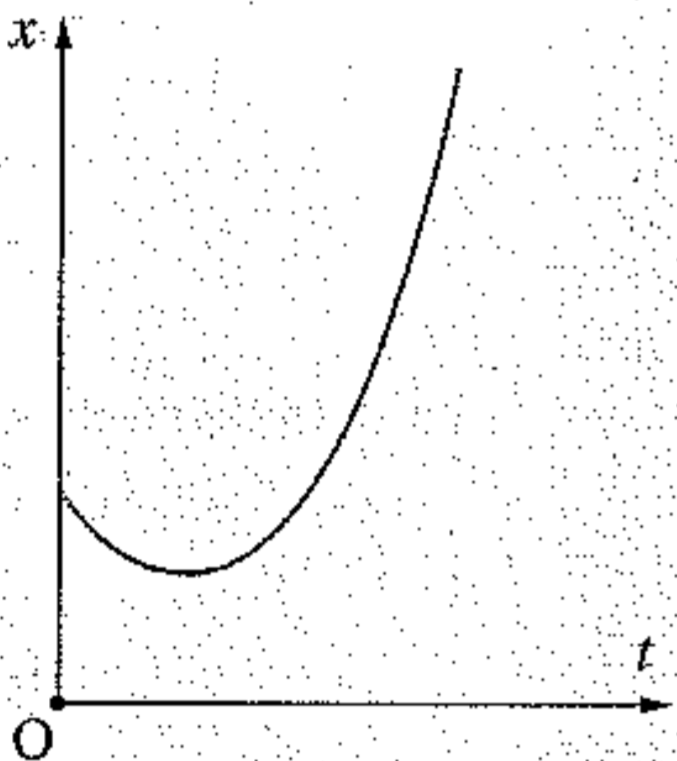
\includegraphics[width=\textwidth]{snelheidsverloop_o}}
%\end{minipage}
%\begin{figure}[H]
%\begin{flushright}
%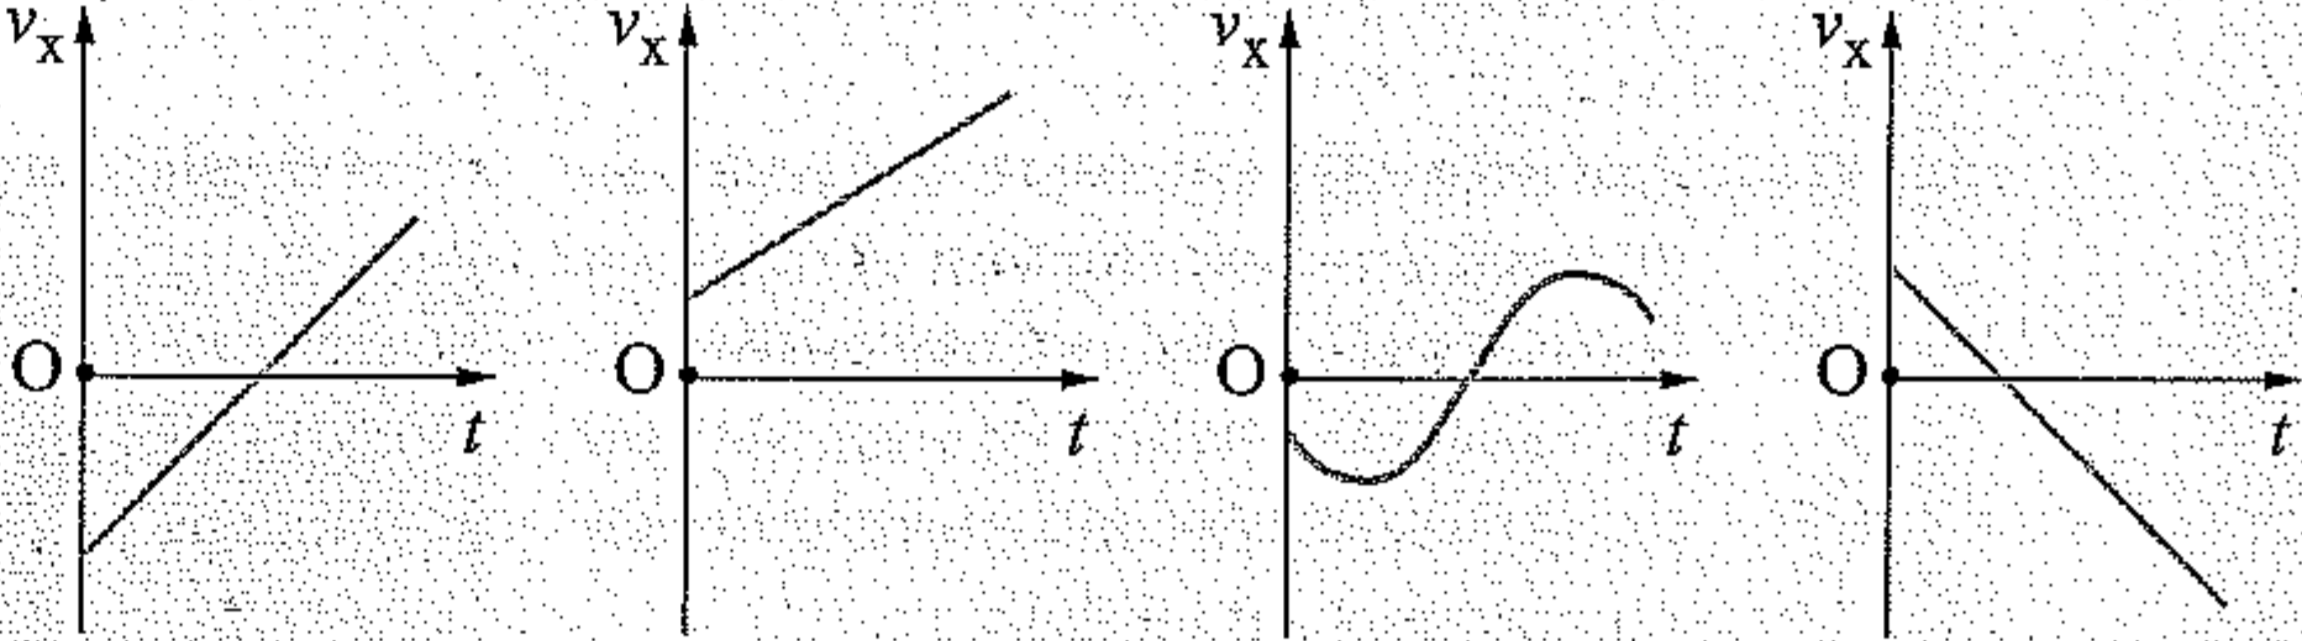
\includegraphics[width=0.93\textwidth]{snelheidsverloop}
%\end{flushright}
%\end{figure}

%\newpage

%\item 
%\begin{minipage}[t]{0.6\textwidth}
%Een deeltje beweegt in de zin van de $x$-as. De nevenstaande grafiek geeft aan hoe de grootte van de snelheid verandert als functie van de tijd.
%\begin{enumerate}
%\item De afstand afgelegd na $15\rm\,s$ bedraagt:
%\newline
%\begin{tabularx}{\textwidth}{XXXX}
%$30\rm\,m$&$120\rm\,m$&$150\rm\,m$&$240\rm\,m$
%\end{tabularx}
%\item Na $30\rm\,s$ heeft het deeltje een welbepaalde afstand afgelegd. Hoe groot zou de constante snelheid van het deeltje moeten zijn om in $30\rm\,s$ dezelfde afstand af te leggen?
%\newline
%\begin{tabularx}{\textwidth}{XXXX}
%$0,0\rm\,m/s$&$§6,0\rm\,m/s$&$8,0\rm\,m/s$&$12\rm\,m/s$
%\end{tabularx}
%\end{enumerate}
%\end{minipage}
%\hspace{2mm}
%\begin{minipage}[t]{0.3\textwidth}
%\raisebox{-5cm}{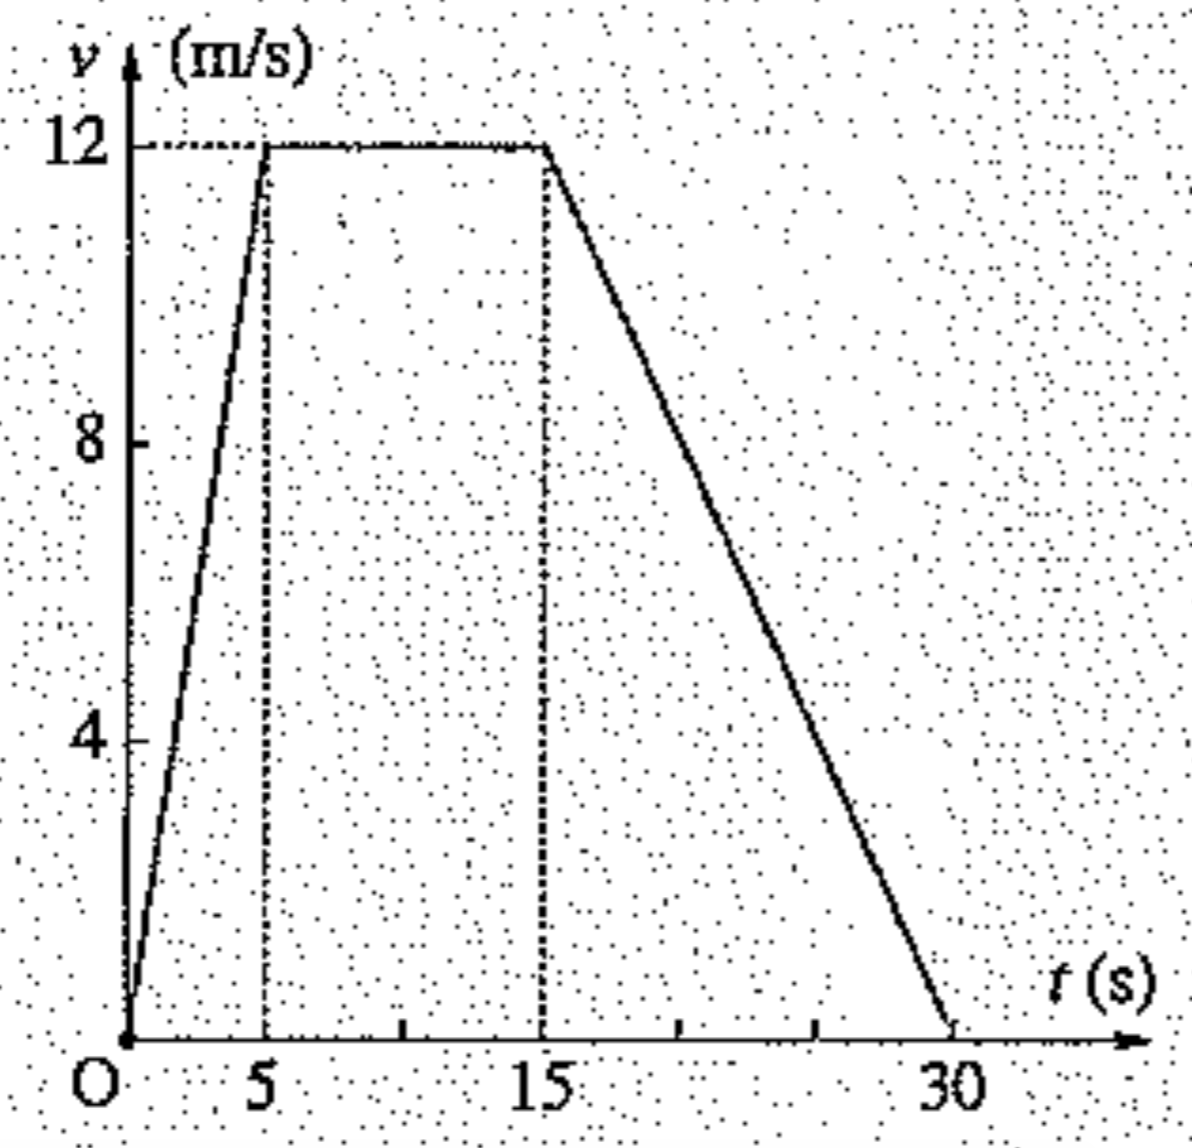
\includegraphics[width=\textwidth]{snelheidsverloop_2_o}}
%\end{minipage}
%\begin{enumerate}
%\setcounter{enumii}{2}
%\item Het verloop van de versnellingscomponent van het deeltje wordt kwalitatief voorgesteld op figuur:
%\begin{figure}[H]
%\begin{flushright}
%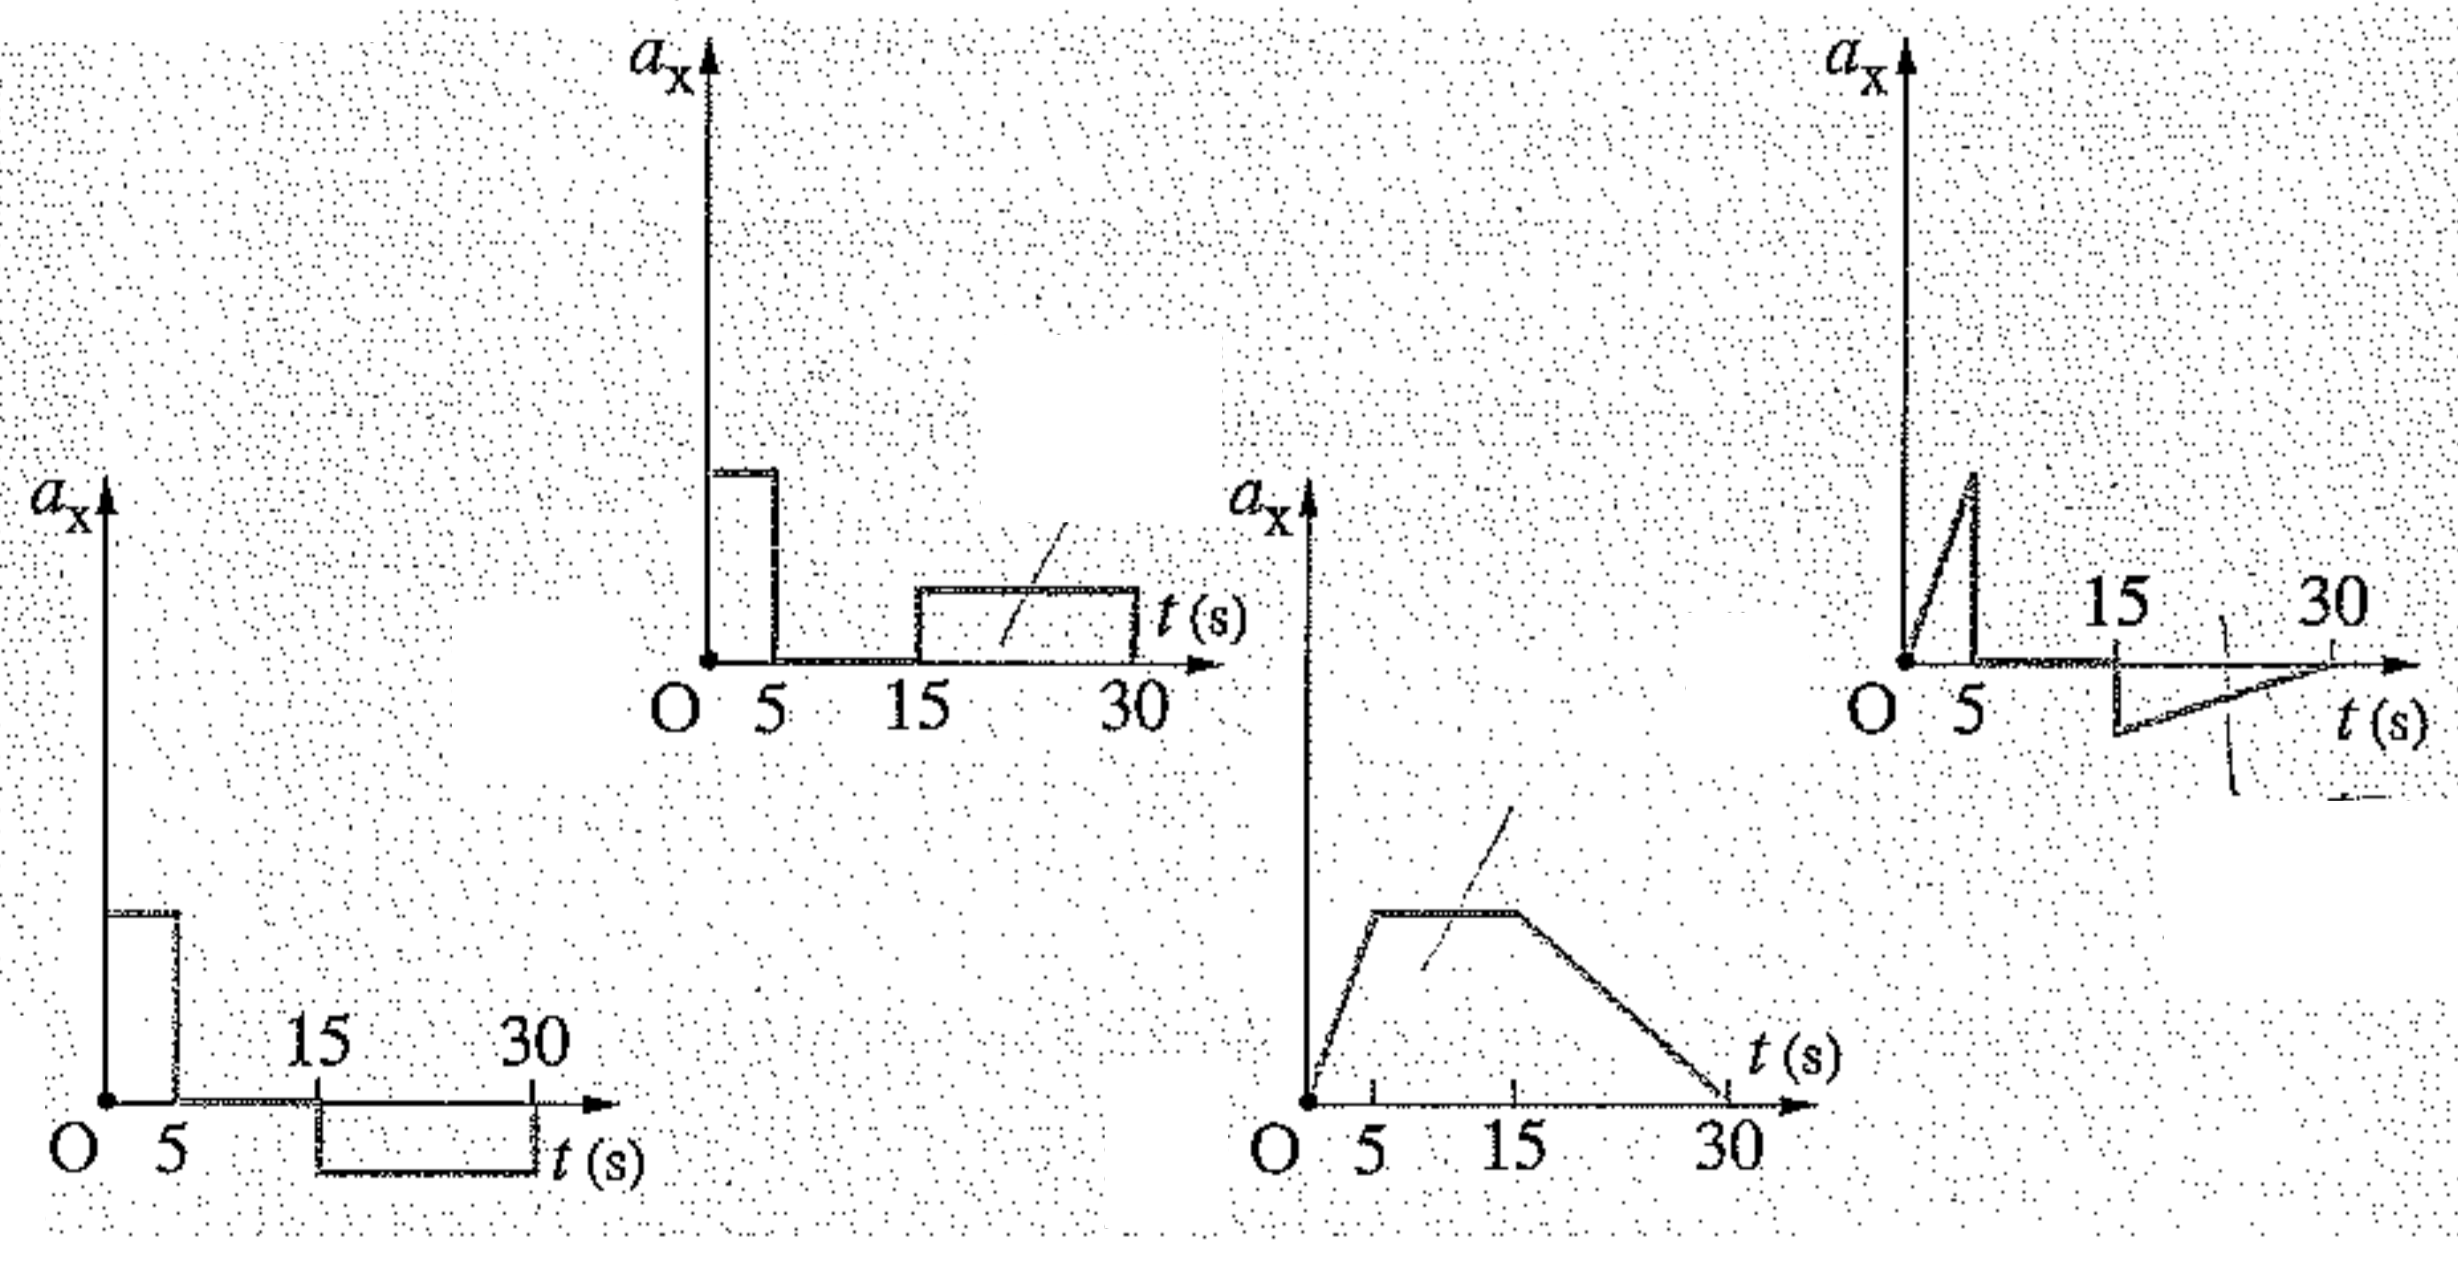
\includegraphics[width=0.93\textwidth]{snelheidsverloop_2}
%\end{flushright}
%\end{figure}
%\end{enumerate}
%
%
%\newpage

% Verticale worp




\item Een appel valt van een boom. Zijn valtijd bedraagt $0,5\rm\,s$. Hoe hoog hing de appel?



\item Vanaf welke hoogte moet een lichaam vrij vallen om met een snelheid van $100\rm\,m/s$ de grond te bereiken?



\item Op het dak van een flatgebouw wordt een bal verticaal
opwaarts geworpen met een snelheid van $10\rm\,m/s$. $4,0\rm\,s$
later bereikt de bal de grond.
\begin{enumerate}
\item Hoe hoog vloog de bal?
\item Hoe hoog is het flatgebouw?
\end{enumerate}

\item Een luchtballon stijgt met een snelheid van $8,0\rm\,m/s$. Op
$100\rm\,m$ hoogte laat men een zakje zand vallen. Hoeveel tijd
heeft het zakje nodig om de grond te bereiken?

\item Uit een luchtballon laten we een steen vrij vallen. E\'en
seconde later werpen we vanuit hetzelfde punt een tweede steen naar
beneden. Wat is de kleinste beginsnelheid die we de tweede steen
moeten geven opdat ze de eerste nog zou kunnen
inhalen?~\footnote{Druk je antwoord uit als functie van de hoogte
$x$. antw.
$v_0=\frac{x-\frac{1}{2}g(\frac{2x}{g}-t_0)^2}{\frac{2x}{g}-t_0}$}

\item Van de boord van een schip valt een loden bol in het water. De
\mbox{boord} bevindt zich $4,0\rm\,m$ boven het wateroppervlak. De
loden bol zinkt vervolgens met de snelheid waarmee hij het water
raakte. Er zijn $6,0\rm\,s$ tussen het tijdstip waarop de bol valt
en ze de bodem van het water bereikt.
\begin{enumerate}
\item Hoe diep is het water?
\item Wat is de gemiddelde snelheid van de bol over het hele
traject?
\end{enumerate}

\item Men laat twee lichamen vallen vanuit rust met een tussentijd van
$1\rm\,s$. Hoe lang na de start van het eerste zijn ze $10\rm\,m$
van elkaar verwijderd? \footnote{antw. $1,52\rm\,s$}

\item Een open liftkooi stijgt met constante snelheid $10\rm\,m/s$.  Een jongen
die in de kooi staat werpt een bal recht omhoog op het moment dat de
lift $30\rm\,m$ boven de grond is. De beginsnelheid van de bal
t.o.v. de lift is $20\rm\,m/s$. zoek de maximale hoogte die de bal
bereikt en hoe lang het duurt voor de jongen hem terug kan opvangen.
\footnote{antw. $76\rm\,m$; $4,1\rm\,s$}



\item Een verticaal vallende steen legt in de laatste seconde, voor hij de grond bereikt, \SI{100}{m} af. Men veronderstelt dat hij vanuit rust vertrok.
\begin{enumerate}
\item Bepaal de snelheid op het ogenblik dat hij de grond bereikt.
\item Bepaal de hoogte vanwaar de steen viel en de tijd die hij daarvoor nodig had.
\end{enumerate}
\begin{oplossing}
\footnote{$v=\frac{x_2-x_1}{t_2-t_1}+\frac{1}{2}g(t_2-t_1)=\frac{\Delta x}{\Delta t}+\frac{1}{2}g\Delta t$
\newline
$t_2=\frac{v_2}{g}=\frac{\Delta t}{2}+\frac{\Delta x}{g\Delta t}$, $x=\frac{1}{2}gt^2=\frac{1}{2g}\left(\frac{\Delta x}{\Delta t}\right)^2+\frac{\Delta x}{2}+\frac{g(\Delta t)^2}{8}$}
\item[\textit{gegeven}]$\Delta t=\SI{1,0}{s}$; $\Delta x=\SI{100}{m}$; $v_0=0$
\item[\textit{gevraagd}]$v_2$, $x_2$, $t_2$
\item[\textit{oplossing}]
\begin{enumerate}
\item 
\begin{minipage}[t]{.7\textwidth}
We kiezen de $x$-as naar beneden zodat de versnelling de valversnelling is, $a=g$. Als we $x_1$ beschouwen als de beginpositie van de beweging die de steen uitvoert in de laatste honderd meter, kunnen we de snelheid vinden waarmee de steen hieraan begint.
\begin{eqnarray*}
&&\Delta x=v_1\Delta t+\frac{1}{2}g\Delta t^2\\
&\Leftrightarrow&v_1=\frac{\Delta x-\frac{1}{2}g\Delta t^2}{\Delta t}
\end{eqnarray*}
\end{minipage}
\begin{minipage}[t][4.5cm][b]{.3\textwidth}
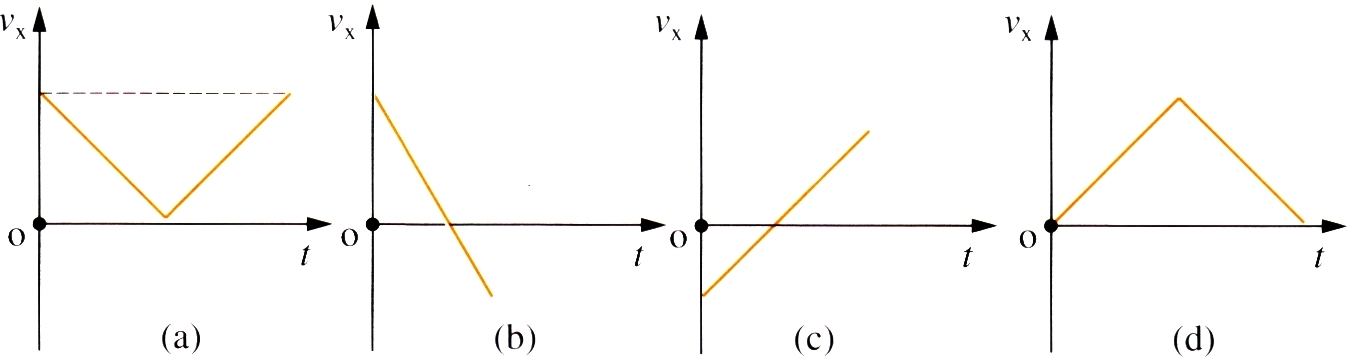
\includegraphics[height=6cm]{valbeweging}
\end{minipage}
\newline
\newline
\newline
Met de formule voor de snelheid van een EVRB, vinden we de snelheid op het einde van het interval.
\begin{eqnarray*}
v_2&=&v_1+g\Delta t\\
&=&\frac{\Delta x-\frac{1}{2}g\Delta t^2}{\Delta t}+g\Delta t\\
&=&\cdots\\
&=&\overline{v}+g\frac{\Delta t}{2}\\
&=&\SI{105}{s}
\end{eqnarray*}
Je kan dit ook afleiden door gebruik te maken van de formule voor gemiddelde snelheid, $\overline{v}=\frac{v_1+v_2}{2}$.
\item Omdat we de snelheid kennen, kunnen we de tijd vinden die de steen nodig heeft gehad om aan deze snelheid te komen. Vervolgens vinden we dan ook de afstand.
\begin{eqnarray*}
t_2=\frac{v_2}{g}=\frac{\overline{v}}{g}+\frac{\Delta t}{2}=\SI{10,7}{s}\\
x_2=\frac{1}{2}gt_2^2=\SI{561}{m}
\end{eqnarray*}
\end{enumerate}
\end{oplossing}



\item Men laat een steentje in een put vallen. Na $10\rm\,s$ hoort
men het de bodem bereiken. Men verwaarloost de tijd die het geluid
nodig heeft om de rand van de put te bereiken.
\begin{enumerate}
\item
\begin{enumerate}
\item Bepaal de snelheid van het deeltje na $5,0\rm\,s$ en na $10\rm\,s$
\item Stel de snelheid grafisch voor in functie van de tijd.
\end{enumerate}
\item
\begin{enumerate}
\item Welk deel van de weg heeft het steentje reeds afgelegd na
$5,0\rm\,s$? Hoe diep is de put?
\item Stel de afgelegde weg grafisch voor als functie van de tijd.
\end{enumerate}
\item Was het in het gegeven toegelaten te onderstellen dat de tijd,
die het geluid nodig heeft om de rand van de put te bereiken, te
verwaarlozen is? De snelheid van het geluid is $343\rm\,m/s$.
\end{enumerate}

\item Iemand gooit vanaf de rand van een klif een steen omhoog met
een snelheid van $10\rm\,m/s$. Na 7 seconden hoort hij de steen in
de oceaan vallen. Hoe hoog is het klif? De snelheid van het geluid
is $343\rm\,m/s$.

\item Iemand aan de rand van een klif laat een steen vallen en hoort
$3,3\rm\,s$ later het geluid waarmee de steen in de oceaan plonst.
De snelheid van het geluid is $343\rm\,m/s$. Hoe hoog is het
klif?~\footnote{$x_0=v_2t_2+\frac{v_2^2}{g}+v_2\sqrt{(t_2g+v_2)^2-t_2^2}$}


\item Schets het $x(t)$- $v(t)$- en $a(t)$-diagram bij een EVRB met $x_0=2,0\rm\,m$, $v_0=20\rm\,m/s$ en $a=-2,0\rm\,m/s^2$.

\item Hieronder worden vier rechtlijnige bewegingen voorgesteld in een grafiek. Dan is de afgelegde weg na $6~\rm s$ het grootst in figuur:
\begin{figure}[h]
\begin{center}
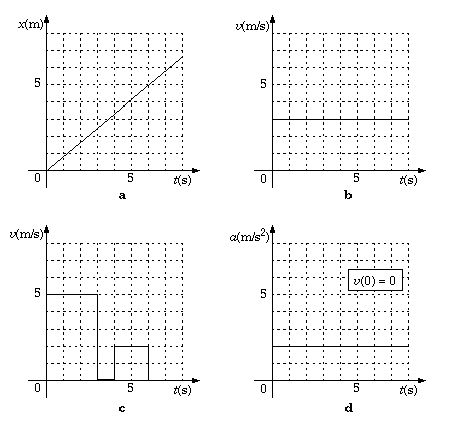
\includegraphics[width=0.8\textwidth, angle=0]{4erbs}
\end{center}
\end{figure}
\footnote{antw. d}


\item De snelheidsfunctie van een auto wordt voorgesteld op de figuur. 
\begin{figure}[h]
\centering
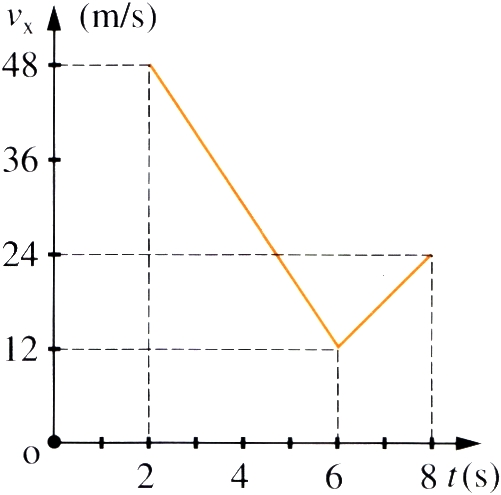
\includegraphics[width=0.32\textwidth]{racewagen}
\end{figure}
\newline
Beantwoord de volgende vragen.
\begin{enumerate}
\item Beschrijf de beweging. 
\item Bereken de positieverandering tussen de tweede en de achtste seconde. 
\item Bereken de gemiddelde snelheid tussen de tweede en de achtste seconde. 
\item Bereken de gemiddelde versnelling. 
\item Teken in de grafiek het snelheidsverloop van een auto die met deze gemiddelde versnelling
zou rijden en op $t=2\rm\,s$ zou beginnen met dezelfde beginsnelheid als de auto in de opgave.
\end{enumerate}



\item In de onderstaande figuur is de positie $x$ van Tieme tijdens een fietstocht
gegeven als functie van de tijd $t$.
\begin{figure}[h]
\begin{center}
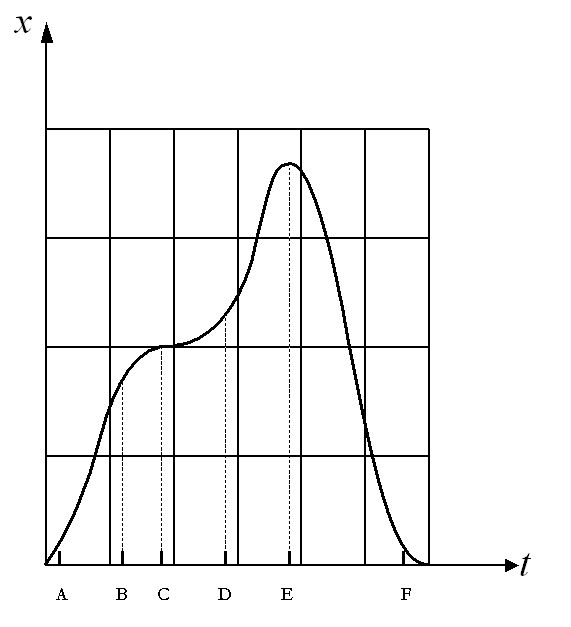
\includegraphics[width=0.4\textwidth, angle=0]{versnelling_xtgrafiek}
\end{center}
\end{figure}
\newline
Welke uitspraak is correct? Op de volgende tijdstippen heeft Tieme
een versnelling die positief is:
\begin{enumerate}
\item C en E
\item B, D en E
\item A, D en F
\item A en D
\end{enumerate}
\footnote{antwoord c}

\item Onderstaande grafiek geeft het
tijdsverloop aan van de positie $x$ van een wagen die met een
constante versnelling vanuit rust vertrekt. Op de verticale as kan
men $x$ aflezen, op de horizontale $t^2$.
\begin{figure}[h]
\begin{center}
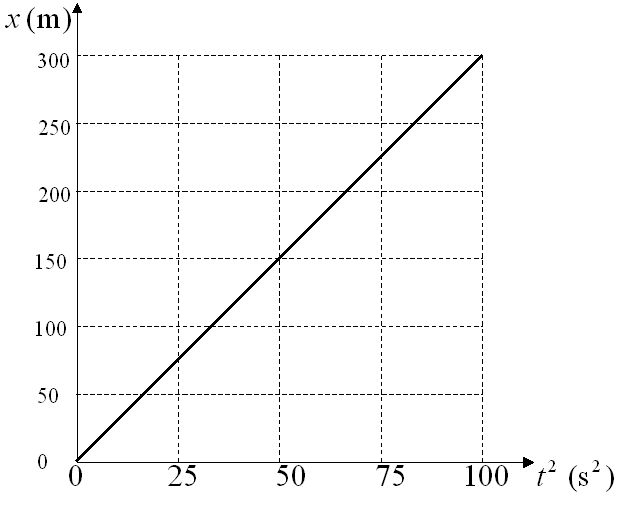
\includegraphics[width=0.4\textwidth]{grafiek_xt}
\end{center}
\end{figure}
\newline
De grootte van de versnelling van de wagen is dan:
\begin{enumerate}
\item 2 m/s$^2$
\item 3 m/s$^2$
\item 6 m/s$^2$
\item 12 m/s$^2$
\end{enumerate}



\item Een bolvormig voorwerp valt verticaal in lucht vanaf een grote
hoogte. De luchtweerstand is \textit{niet} te verwaarlozen. De
beweging wordt het best weergegeven door de figuur:
\begin{figure}[h]
\begin{center}
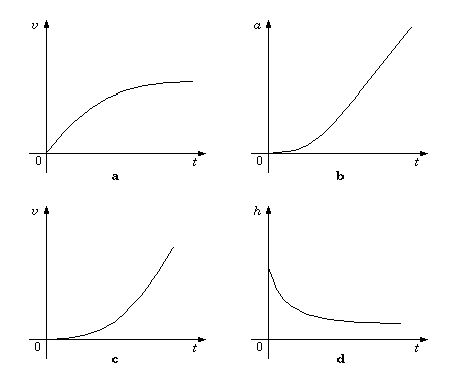
\includegraphics[width=0.8\textwidth, angle=0]{vallend_voorwerp_wrijving}
\end{center}
\end{figure}
\footnote{Antwoord (a) is juist.}

\begin{oplossing}
\item De snelheid waarmee de patrouilleleider vooruit gaat, is de snelheid waarmee de $x$-co\"ordinaat verandert. De snelheid waarmee het mandje omhoog gaat, is gelijk aan de de snelheid waarmee de lengte $l$ langer wordt. Dus
\begin{eqnarray*}
v&=&\frac{dx}{dt}\\
v'&=&\frac{dl}{dt}.
\end{eqnarray*}
Nu zijn de lengte $l$ en de positie $x$ aan elkaar gerelateerd via de stelling van Pythagoras, $l^2=x^2+h^2$. De lengte $l$ is dus te schrijven in functie van $x$: $l=\sqrt{x^2+h^2}$. Nu zijn zowel $l$ als $x$ functies van $t$ en kunnen we $l(t)$ als een samengestelde functie beschouwen:
\begin{eqnarray*}
l(t)=\sqrt{\left(x(t)\right)^2+h^2}
\end{eqnarray*}
Wanneer we $l$ willen afleiden, moeten we dus de kettingregel\footnote{Merk op dat we hier met drie samenstellende functies te maken hebben. Eerst wordt $t$ afgebeeld op $x(t)$, vervolgens wordt $x$ afgebeeld op $x^2+h^2$ en de laatste functie in de schakel is de wortelfunctie.} gebruiken.
\begin{eqnarray*}
\frac{dl}{dt}&=&\frac{dl}{dx}\frac{dx}{dt}\\
&=&\frac{2x}{2\sqrt{x^2+h^2}}\frac{dx}{dt}\\
&=&\frac{x}{\sqrt{x^2+h^2}}v
\end{eqnarray*}
De uitspraak met de vectoren is fout omdat de snelheden een verschillende richting hebben
\end{oplossing}

\end{enumerate}













